%
% File hicss51.tex
%
% Contact: Holm Smidt, hsmidt@hawaii.edu
%%
%%
%% Based on the style files for ACL 2015 by 
%% car@ir.hit.edu.cn, gdzhou@suda.edu.cn


\documentclass[10pt]{article}
\usepackage[letterpaper]{geometry}
\usepackage{hicss51}
\usepackage{times}
\usepackage[none]{hyphenat}
\usepackage{url}
\usepackage{latexsym}
\usepackage{minted}
\usepackage{indentfirst}
\usepackage{graphicx}
\graphicspath{{images/}}

\usepackage{blindtext}
\usepackage{amsmath}
\usepackage{eurosym}
\usepackage{textcomp}
\usepackage{multicol}
\newcommand{\sansserifformat}[1]{\fontfamily{cmss}{ #1}}%




%\setlength\titlebox{5cm}

% You can expand the titlebox if you need extra space
% to show all the authors. Please do not make the titlebox
% smaller than 5cm (the original size).


\title{Improving Bus Schedules and Waste Collection Routes \\ in Practical Smart City Implementations}

\author{
  Jan D{\"u}nnweber  \\
  Ostbayerische Technische \\ Hochschule Regensburg \\
  {\underline{ jan.duennweber@othr.de} }\\\And 
  Amitrajit Sarkar \\
 Ara Institute \\ of Canterbury \\
  {\underline{amit.sarkar@ara.ac.nz}} \\\And
  Vimal Kumar Puthiyadath \\
 KPIT Technologies Ltd \\
  {\underline{Vimal.Puthiyadath@kpit.com}} \\\And
  Omkar Barde \\
 KPIT Technologies Ltd \\
  {\underline{Omkar.Barde@kpit.com}} 
 }

\date{}
% \makeatletter
% \renewcommand*{\@seccntformat}[1]{%
%   \csname the#1\endcsname\quad
% }
% \makeatother

\begin{document}
\maketitle
\begin{abstract}
Computer-based Improvements of waste collection and public transport procedures are 
often a part of smart city initiatives. When we envision an ideal bus, it will 
primarily connect the most crowded bus stops. Similarly, an ideal waste collection 
vehicle will arrive at every container exactly at the time when it is fully loaded. 
Beyond doubt, this will
reduce traffic and support environmentally friendly intentions like an expansion
of waste separation, as it will make more containers manageable.
An obvious difficulty of putting that vision into practice is that
vehicles cannot always be where they are needed.           
Knowing the best time for arriving at a certain position is insufficient for 
finding the optimal route.
Therefore, we compare four different approaches to optimized routing: 
Regensburg, Christchurch, Malaysia and Bangalore. Our analysis shows 
that the most efficient schedules           
result from adapting field-tested routes frequently on the basis of
sensor measurements and shortcuts resulting from route        
optimizing computations.
\end{abstract}

\section{Introduction}
Even with the latest IoT technology like networked sensors and simulations
forecasting the behaviour of the population of megacities, practical implementations 
of on-demand public transport and smart waste collection still have difficulties 
in keeping up with the prognosticated improvements.
A vehicle that drives obstinately from the most crowded bus stop (respectively, the 
most heavily filled container) to one with the fill-grade closest 
to that will obviously need more time in the majority of cases than a vehicle 
following a fixed plan, 
since the crowded bus stops and the heavily filled containers are probably 
positioned far apart from 
each other. 

Finding a smarter route leads us to the classic 
{\it vehicle routing problem} (VRP~\cite{Dantzig59}), an instance of the 
{\it Travelling Salesman Problem (TSP)} with the added constraint that we 
need to return to the starting point after visiting a fixed number of points, 
since the collection vehicle has a limited capacity. 
Thus, we don't need to find the minimum Hamiltonian
circle through all the points but multiple circles forming some kind of
clover leaf. However, finding the best route does not only require to consider the distances between the single stops. Busses should leave out stops where no
passengers are waiting and waste collectors should skip containers which are filled only 
to a certain level, i.\,e. we are dealing with an instance of a dynamic route 
planning problem, which is also the subject of more recent 
research~\cite{Chen16}.

There are $\frac{n!}{2}$ different routes connecting $n$ positions. 
For comparing all possible routes between only $10$ stops, this means 
3628800 routes must be analyzed. While a typical bus line might 
comprise $10$ stops, a modern waste collection
vehicle can be loaded with $\approx 400$ containers of 120 
liters~\cite{hyundai18}.
$400!$ is a $882$-digit number. 
%, i.\,e. finding the best route 
% for the waste collection using a brute force program is inconceivable. 
Skipping 
containers with little load means, the vehicle has to pickup an other
one, where it usually does not drive to. Thus, solving the dynamic VRP 
requires to solve a new problem of that size, every time when the fill level
measurements are updated. Nowadays, supercomputers can deal with 
such problem sizes~\cite{Burkhovetskiy2017}. However, this work 
presents four projects based on approximate solvers, which
can run a standard PC or an on-board computer. % in a bus or garbage truck. 
Therefore, the presented work is relevant 
for automating the navigation of autonomous busses and robotic garbage 
trucks, like the one Volvo started testing in Brussels 
recently~\cite{volvo17}.


The rest of this paper is structured as follows: 
Section~\ref{sec:aco} explains the {\it ant colony optimization} (ACO)
% for solving VRP instances appoximately 
and shows how %the cities 
Regensburg 
and Christchurch benefit from ACO and fill level sensing for collecting 
their waste containers. 
Section~\ref{sec:kpit} introduces a different approach to minimizing routes
be means of a greedy algorithm and shows two more practical implementations:
The waste collection in Malaysia and the employee transport service of 
Bangalore.
Section~\ref{sec:concl} %looks back on the four projects,
% which were all put into practice, 
discusses the lessons learned %from these projects,
%their benefits 
and points out some future perspectives.

\section{Intelligent Routing by means of the Ant Colony Optimization (ACO)}
\label{sec:aco}

The {\it ant colony optimization} is an approximate solution for TSP
instances (ACO~\cite{Dorigo97}). This 
approach has also been proven suitable for dynamic VRP instances
in a simulation, where the road network and the related 
traffic were taken into account~\cite{Karadimas2008}. ACO is a {\it swarm intelligence}
procedure, i.\,e. not an individual (a simulated ant in the case of 
ACO) solves the problem but a group. For finding optimal routes,
the simulation starts with letting the ants take random paths
until they reach their destination. This random walk is optimized
iteratively: each ant leaves a pheromone trail behind it which
evaporates after a certain number of iterations. In every iteration
the pheromone intensity of the shorter paths increases because
whenever a simulated ant can choose among multiple paths, it takes
the one with the highest pheromone intensity. This means, in higher
iterations, the paths are no more randomly chosen but influenced 
by the most successful ants from preceding iterations. These are
the ants whose pheromone trails did not evaporate until their 
followers reached them, since they were on the shortest paths.


\subsection{Application 1: The Collection of Biological Waste in Regensburg}
\label{sec:Regensburg}

Our work in Regensburg focuses on improving the collection of biological waste~\cite{Burger18}.
While other approaches toward the computer-aided routing of waste collection vehicles 
rely only on fill level sensing~\cite{LundinOS17} or only on ACO-based path 
computations~\cite{ismail09}, we combined both ideas. 

\begin{figure}[h!]
  % Use the relevant command to insert your figure file.
  % For example, with the graphicx package use
    \centering
  \includegraphics[%trim={3cm 4cm 3cm 3cm}, clip,
  width=0.95\linewidth]{electricbin}
  % figure caption is below the figure
  \caption{Container (left) and electronics (right)}
  \label{fig:container}       % Give a unique label
\end{figure}

Simulations have shown, that 
the combination of these techniques can significantly reduce the time needs for the collection
of waste~\cite{Sharmin16}. A comparison of related projects shows that most route optimization projects for the collection of waste lead to the development of a 
computer simulation~\cite{likotiko17}. The reasons which prevented the incorporation
of this work in practical smart city implementations were, amongst others,  
present contracts with service providers and logistical
obstacles conflicting with changes to the waste collection routes. Possible time savings could only be computed but not really be exploited in many places.

\subsubsection{Practical implementation}

In Regensburg, we recently started applying route optimization and fill level 
sensing to the collection of the containers for biological waste.
Figure~\ref{fig:container} (left) shows one such container and the protection casing on the
back which houses our electronics. Actually, the
right part of the picture with the detail view of the electronics shows an 
earlier prototype
where the electrical parts were placed in the lid. The new box is smaller (making it more difficult
to recognize single parts like our LoRa transmitter) and delivers correct data, even 
if the lid of the container 
is not properly closed.

\begin{figure}[h!]
  % Use the relevant command to insert your figure file.
  % For example, with the graphicx package use
    \centering
  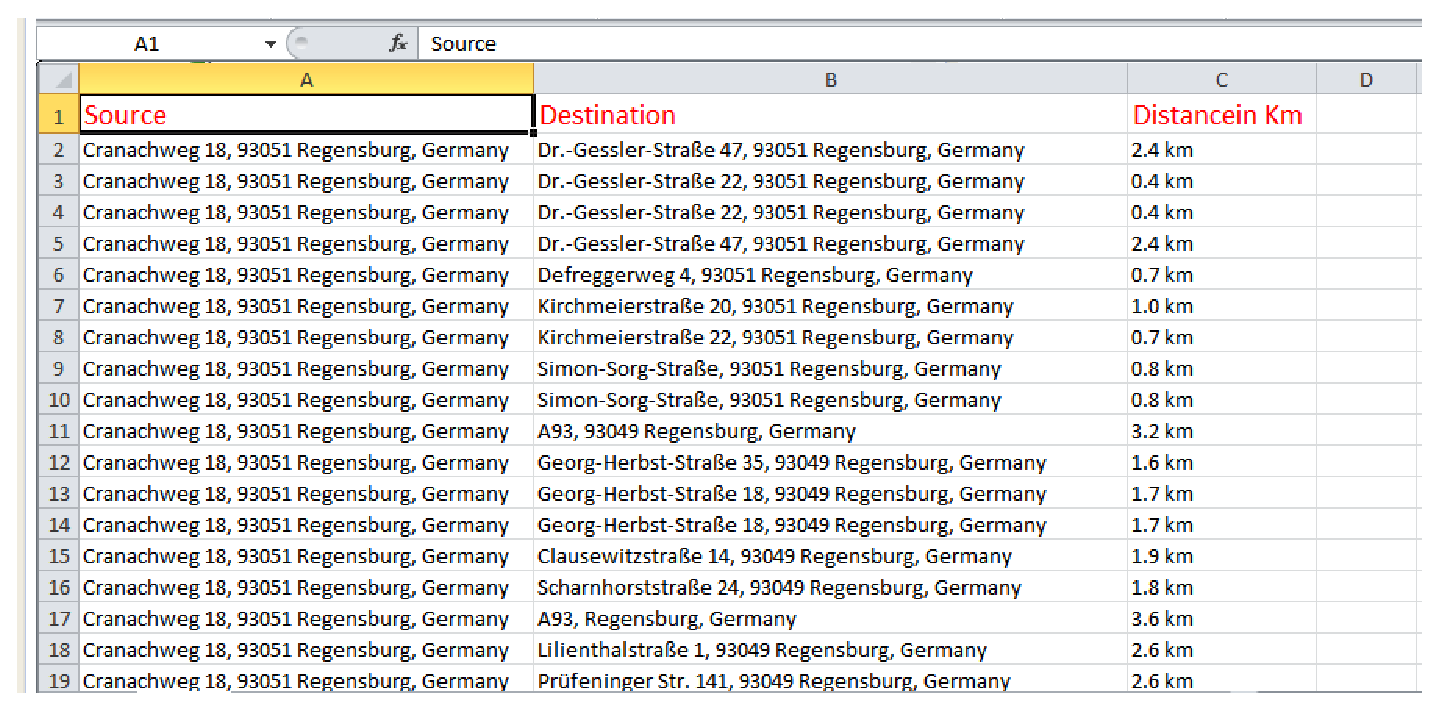
\includegraphics[%trim={3cm 4cm 3cm 3cm}, clip,
  width=0.95\linewidth]{excel}
  % figure caption is below the figure
  \caption{Distances in an Excel sheet}
  \label{fig:excel}       % Give a unique label
\end{figure}

Regensburg established its novel program for the collection of biological waste in 2018.
The city and its surrounds were equipped with 700 new containers. The novelty of the program
allows us, computer scientists (headed by author Jan D{\"u}nnweber) and electrical 
engineers (headed by his colleague Martin Schubert) at the {\it Technical 
University of Applied Sciences} in Regensburg (OTH), to contribute to the
implementation.
Noteworthy as well, is that 700 containers are not too many. While the number
of possible thorough paths, connecting all containers is tremendous ($\frac{n!}{2}$ is a 
1719-digit number), there are only  $\tbinom {700}{2}$ ways to choose an interconnecting 
route between an unordered pair of containers. Numerically, there are 
%\\ \begin{center}
$\frac{700!}{2!(700 - 2)!}= 
\frac{700!}{2 \times (698)!}=\frac{699 \times 700}{2}=
244650$ %\end{center} 
possible interconnections. The Combinations may vary, but the 
single interconnections are static and can be stored in a file (like 
shown in Figure~\ref{fig:excel}) or database.

\subsubsection{Preliminary work}

We set up a database, which holds for half of the 700 containers ({\it one-way})
a file with the distances connecting it to the remaining 699 candidates.% 
% (244650 entries totally).

To ascertain the profitability of our undertakings, we also started with a simulation.
However, our simulation did not forecast the profit from using ACO on arbitrary 
routes or the benefits from observing arbitrary containers. We computed a viable 
forecast for 
Regensburg (see section~\ref{sec:predict}).
With the help of a group of students (David Burger, Vadim Dechand, 
Haris Shehzad and Markus Wildgruber), we could fill the mentioned 
244650-entry database with concrete distances and average driving times. 
Figure~\ref{fig:excel} shows the first 19 entries of this database (in an
Excel-sheet). Actually, we maintain this data in Redis to benefit from caching
when the same interconnection distances are requested repeatedly~\cite{Carlson13}. 

After accompanying
the waste collectors and recording the GPS positions of the containers and the time needs 
for emptying them with a fitness tracking app on the smart phone, we requested the
distances for all possible pairs from the {\it Google Maps} Web service by means of a 
Java program, which the students have developed to export the distance data into the
popular TSPLIB-format~\cite{tsplib90}. With this representation, our data can be 
processed using Open-Source ACO-code and other TSP-solvers. Our routing software makes
use of the Thomas St{\"u}tzle Implementation~\cite{Dorigo97} and we used the exact 
TSP-solver {\it Concorde}~\cite{applegate01} as a reference. 
The recorded data and container-specific properties, such as the distance of
a container to the city center and the number of neighboring containers, helped 
us to determine realistic probabilities for the containers to be empty at collection
time in our simulation. The resulting forecasts were used to select the first 
10 containers which we equipped with real electronics.
Figure~\ref{fig:optmap}
shows the route we computed for connecting 10 containers in red. This route is 
11 kilometers long and could be shortened to 7 kilometers (green route) after
leaving out two containers, which we identified as empty containers using 
our fill level sensors.

\subsubsection{Overfull and Underfull Containers}

\begin{figure}[h!]
  % Use the relevant command to insert your figure file.
  % For example, with the graphicx package use
    \centering
  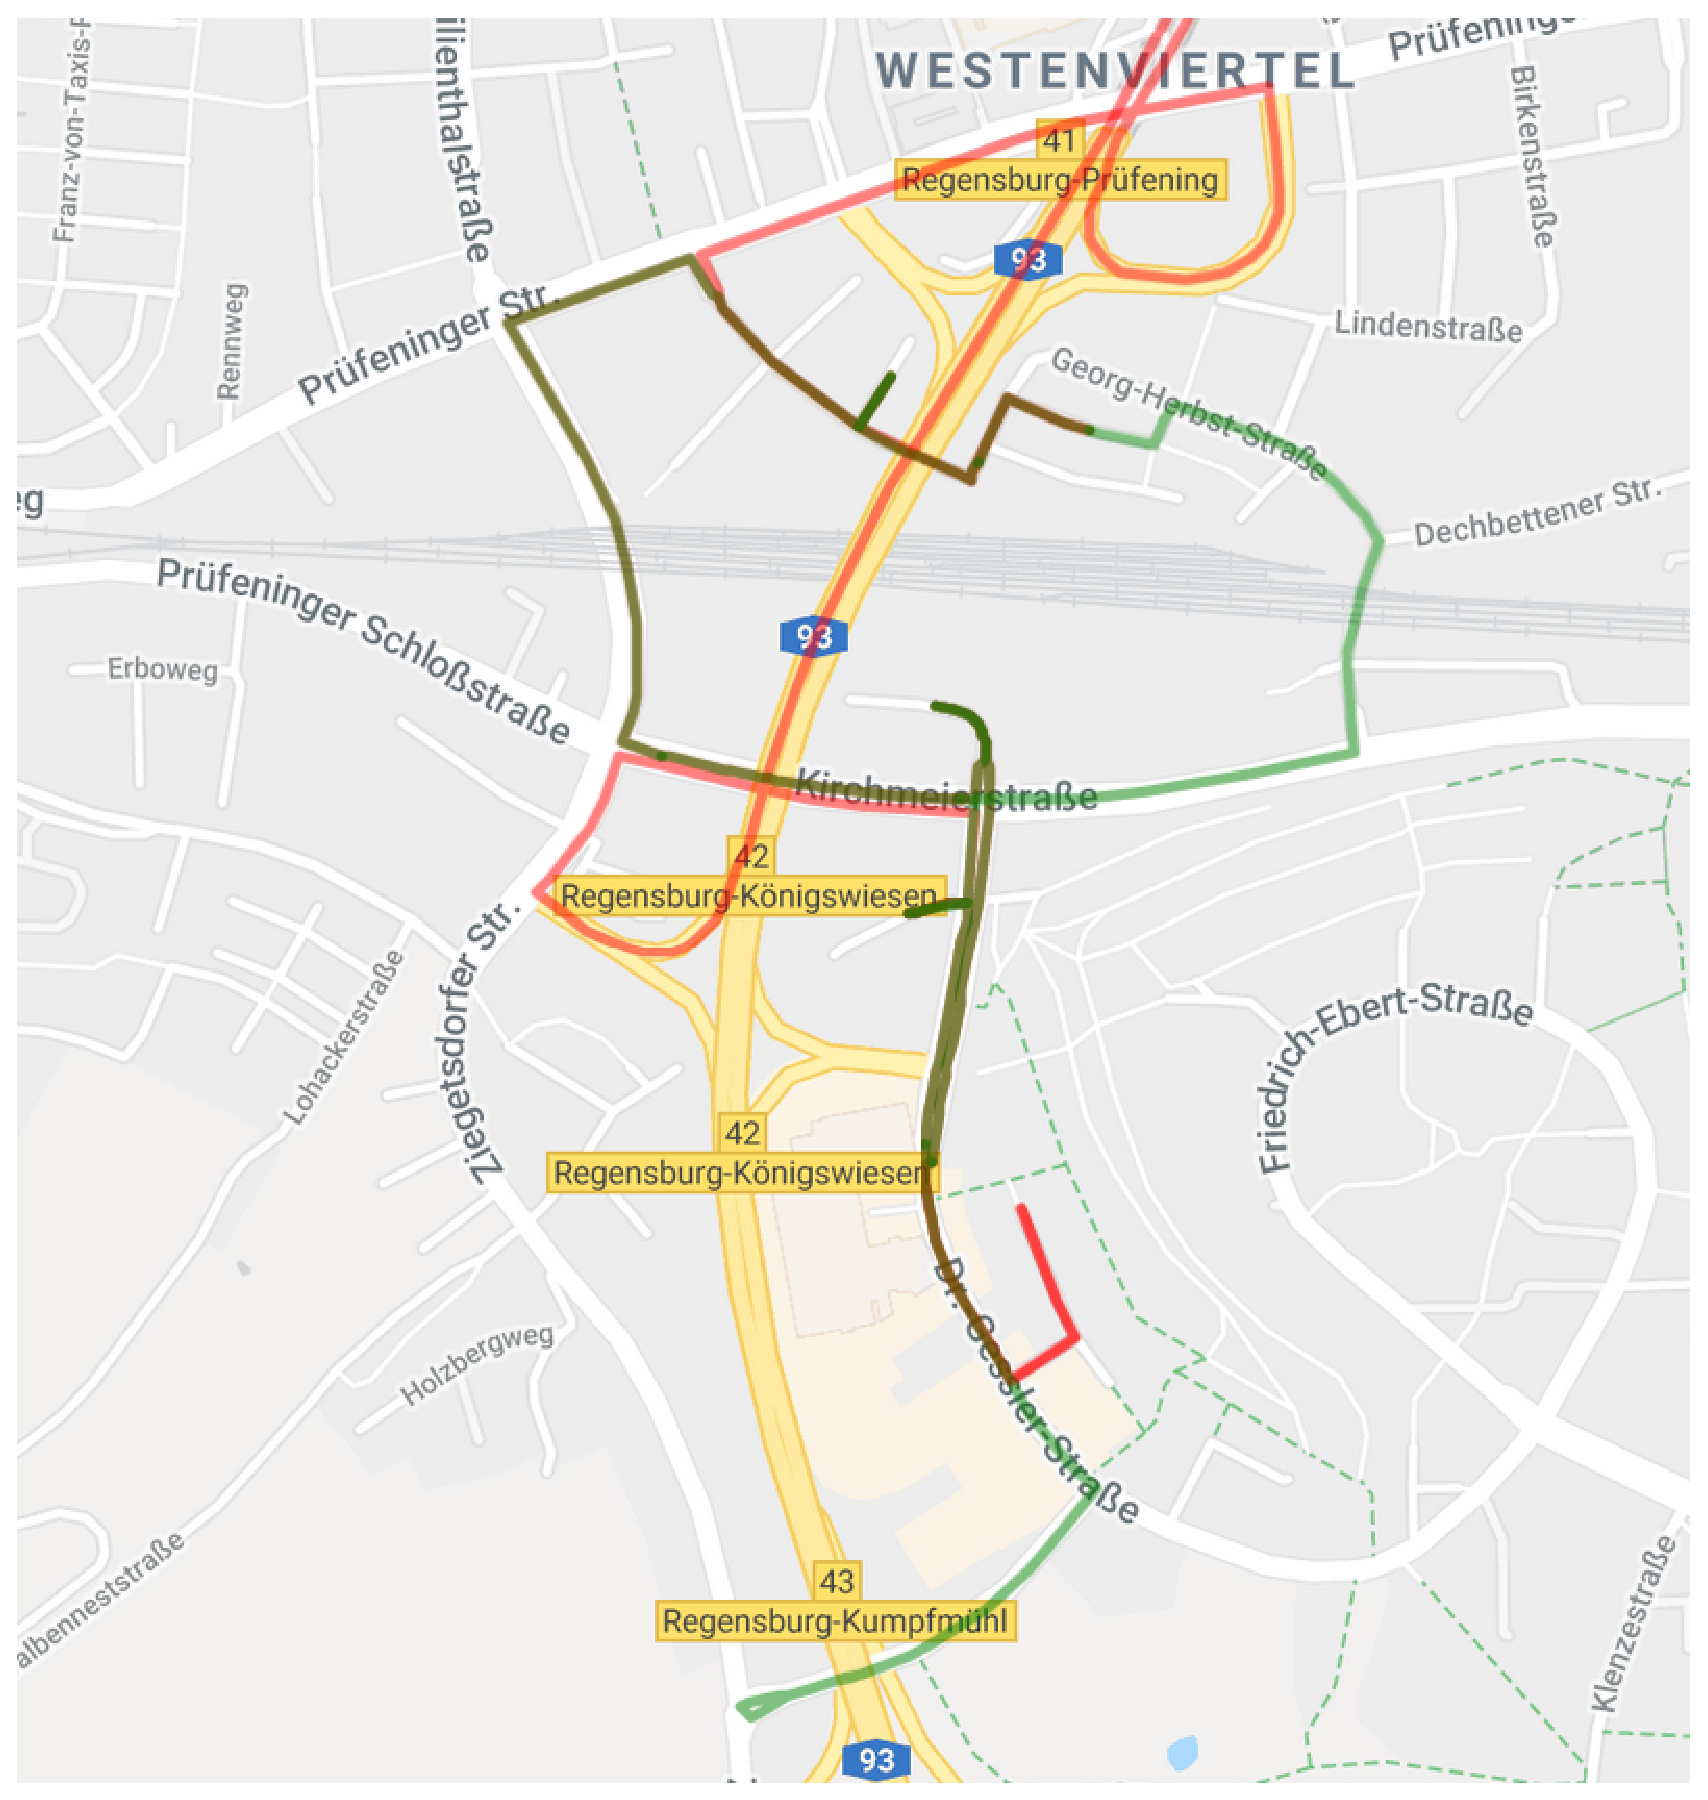
\includegraphics[%trim={3cm 4cm 3cm 3cm}, clip,
  width=0.95\linewidth]{optmap}
  % figure caption is below the figure
  \caption{Original (red) and optimized (green) container collection route}
  \label{fig:optmap}       % Give a unique label
\end{figure}

To integrate fill-level sensing with the ACO-based route computations, we started 
to cope with
underfilled containers. While overfilled containers seem to be 
a more urgent problem, it is difficult (or almost impossible) to send a vehicle  
instantaneously, when an overfilled container is detected. Planning collection 
routes such that underfilled containers are skipped is much easier and saves time and
the saved time is used to collect new containers. The recorded data about
overfilled containers helps the Regensburg city council with positioning the new 
containers where they are needed.
Thus, our waste management software, tackles both problems, underfilled containers directly
(by leaving them our during the collection) and overfilled containers as well, 
by finding the best positions for new containers in the long run. Instead of
resetting the route computations when a container is added, removed or 
re-positioned, we keep the ACO software continuously running, since it is known that the 
swarm algorithm adapts to its input~\cite{angus2005}.

Master-student Josef Wei{\ss} (from Martin Schubert's group) set up the electronics
shown in Figure~\ref{fig:container}: The larger board (on the right) holds an ultrasonic transceiver module and a low power µC. The smaller board holds and a 
LoRa (Low Range) transceiver. We communicate the fill grade measured by the 
ultrasonic transceiver via a LoRa gateway. The total costs for our first 10 
{\it DIY}-devices 
were below $1000$~\EUR{} and sponsored by our project partner {\tt kpit.com}.

\subsubsection{Fill Level Prediction}
\label{sec:predict}

Using our simulation, we could predict that 10 sensors are enough to start
benefiting from our software. To compute a trustworthy prediction, our simulation
does not simply roll the dice to decide whether a sensor-equipped container can
be skipped. Instead the probability for each container $i$ to be empty was 
computed individually using the formula: $P(x_i)=q_i* \frac{c_i}{d_i}$. The value for 
$q_i$ ranges between $0.1$ (overfull), $0.2$ (full), $0.3$ (half-full) and $0.5$ (empty)
and was set accordingly to the average fill level of that container which we observed on
the collection tours. Parameter $d_i$ takes account for the fact that waste containers 
located near the city center are more likely found full and is $1.2$ for a container
withing a $2$ kilometer circle around the center; $1.1$ withing $4$ kilometers and $0.9$ for 
containers located more than $6$ kilometers away from the center. Parameter $c_i$ is weighted 
accordingly to the number of waste containers next to it and $0.9$ when there is none; 
$1.1$ for up to $5$ neighboring containers and $1.3$ for $6$ or more.
With these estimations, we predicted time savings of approximately one hour per day.
Regensburg has just started to adapt the routes accordingly. Thus, we will soon
know how many extra containers can be emptied within the saved time.

\subsection{Application 2: LevelSense\texttrademark ~and PiP-IoT}
\label{sec:Christchurch}

Smart garbage collection is only a part of a larger smart city initiative in
New Zealand which comprises efficient street and traffic lighting, 
water and wastewater management and energy-saving as well.
New Zealand may be considered a small country, but its smart city ambitions are 
anything but small. For the last two consecutive years New Zealand earned a remarkable amount of honors for its smart cities innovations in the annual Smart City Asia Pacific Awards (SCAPA), a competitive benchmarking program conducted by Council Associate Partner IDC.
In reply to the disastrous earthquakes of 2010/11, Christchurch City Council (CCC) put aside funds for ‘Sensing Cities’ initiatives. In November 2015, the Smart Cities programme was initiated to carry out rapid proof of concept projects.

With 3 more years background, the Christchurch projects are a bit
more advanced than the work in Regensburg and the results matter beyond the 
borders of New Zealand: More than 50\% of the world’s population lives in cities by 2050, it will be more the 75\%. While the world’s cities only cover two per cent of the global land area, they are responsible for 70\% of greenhouse gas emissions and the global climate change.
As a consequence, we urgently need sustainable solutions to combat these city-focused issues. The reduction of $CO_2$ emissions from motor vehicles are all essential elements of these solutions. 

\subsubsection{A Versatile Level Sensor}

Christchurch is using smart sensors to ensure that rubbish bins are emptied at 
the right time. 

\begin{figure}[h!]
  % Use the relevant command to insert your figure file.
  % For example, with the graphicx package use
    \centering
  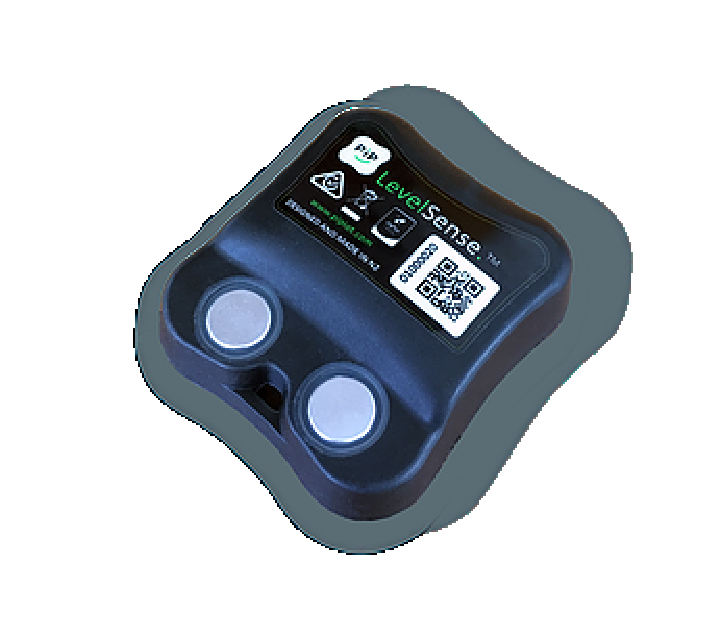
\includegraphics[%trim={3cm 4cm 3cm 3cm}, clip,
                   width=0.695\linewidth]{levelsense}
  % figure caption is below the figure
  \caption{The CCC waste bin sensor}
  \label{fig:levelsense}       % Give a unique label
\end{figure}

Figure~\ref{fig:levelsense} shows one of the LevelSense\texttrademark ~devices.
The LevelSense\texttrademark ~product was developed by Christchurch company PiP IoT to check rubbish levels. The sensors allow city council’s contractors to recognise optimal waste collection times. Its key features are
\begin{itemize}
\item Tilt sensing 
\item GPS position and movement monitoring
\item Tampering and orientation detection
\item Shock and vibration sensing
\item Temperature measurement
\item An expected battery life of 5 years
\item Low power network / LPWAN connectivity
\item Real time analytics
\item Mobile / Web reporting
\item SIGFOX class 0 certification
\end{itemize} 

\subsubsection{Project Outcomes}

Christchurch's rubbish collection contractors work constantly to empty the city's bins 
but when they arrived at a bin, before the introduction of LevelSense\texttrademark, they did not know whether it was empty, full one or an overflowing mess. 
PiP IoT developed LevelSense\texttrademark ~primarily to avoid overflowing public 
rubbish bins, which where a frequent source of complaints from residents.
Though, with the LevelSense\texttrademark ~devices, multiple other enhancements 
are anticipated.

\begin{itemize}
	\item
	A reduction of CO2 emissions and pollution: Fewer rubbish collection trucks on the road for less time means lower fuel consumption and lower greenhouse gas emissions. Fewer collection trucks on the road will also mean less noise pollution, air pollution, and less wear and tear on the road network.
	\item
	A reduction in operational costs: Managing waste takes a large portion of our rates. Bin level sensors and monitoring solutions have been known to reduce waste collection costs by up to 50 \% (fewer collections mean less money spent on driver hours, fuel and truck maintenance).
	\item
	Improved hygiene: overflowing rubbish is a breeding ground for bacteria, insects and pests because of accumulated rubbish. It’s a public nuisance and unpleasant for residents and tourists.
	\item
	Identification of misuse of public rubbish bins: for example, sudden spikes in rubbish levels at night can indicate that household rubbish is being dumped illegally from residents or campers. 
\end{itemize}

\subsubsection{The PiP IoT mobile waste monitoring App}

Christchurch selected the local company PiP IoT to develop and test sensor and
software technology % in the combat against overflowing rubbish bins 
with the objective of creating operational efficiencies and an enhanced streetscape for citizens.

\begin{figure}[h!]
  % Use the relevant command to insert your figure file.
  % For example, with the graphicx package use
    \centering
  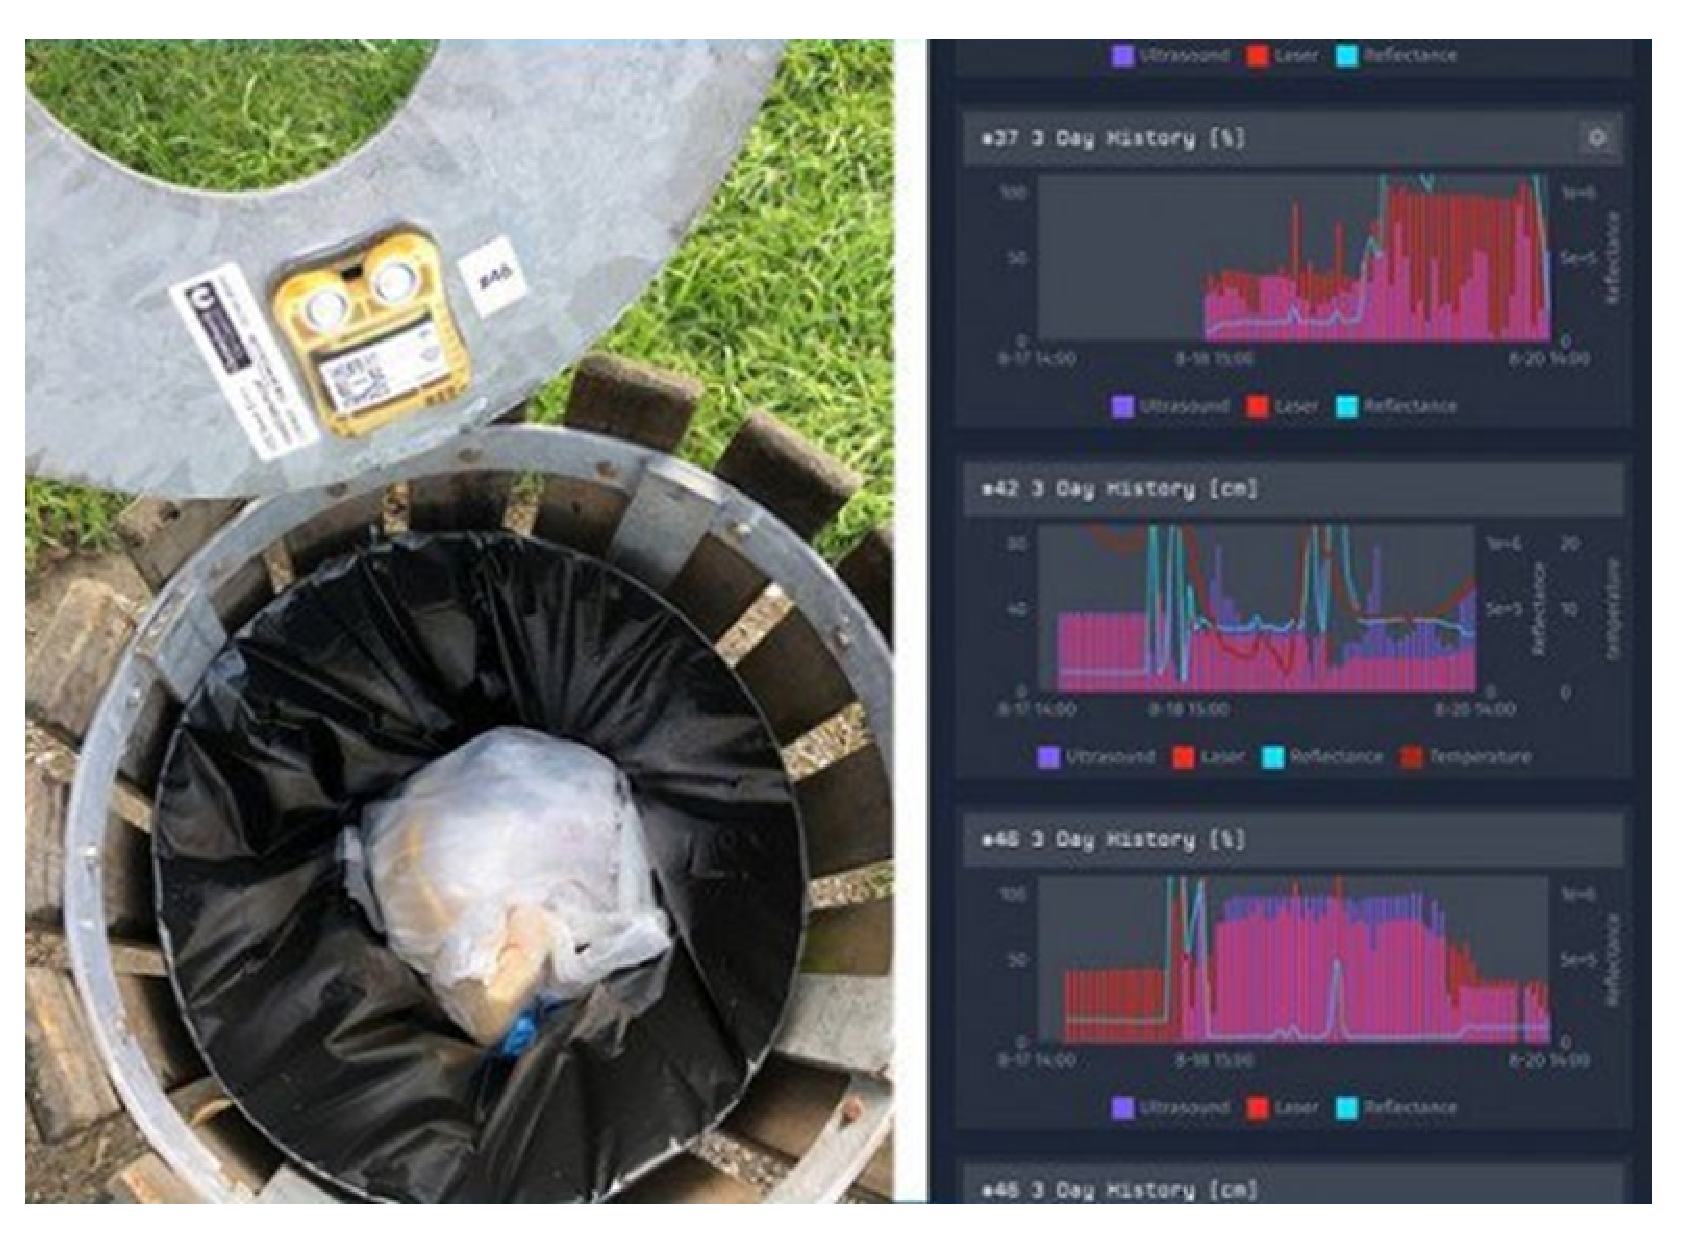
\includegraphics[%trim={3cm 4cm 3cm 3cm}, clip,
                   width=0.95\linewidth]{binmon}
  % figure caption is below the figure
  \caption{LevelSense\texttrademark ~in container lid (left) 
           and the Christchurch online monitoring app (right)}
  \label{fig:binmon}       % Give a unique label
\end{figure}


PiP IoT has rolled out LevelSense\texttrademark ~devices to bins around rubbish trouble spots, including a city park and a retail area. Notifications are sent to contractors’ phones and bin status across the city can be viewed in an online dashboard telling them how full each bin is (see figure~\ref{fig:binmon}, right). Rubbish levels are also being tracked, providing a graphic illustration of when the bins are used most.

\begin{figure}[h!]
  % Use the relevant command to insert your figure file.
  % For example, with the graphicx package use
    \centering
  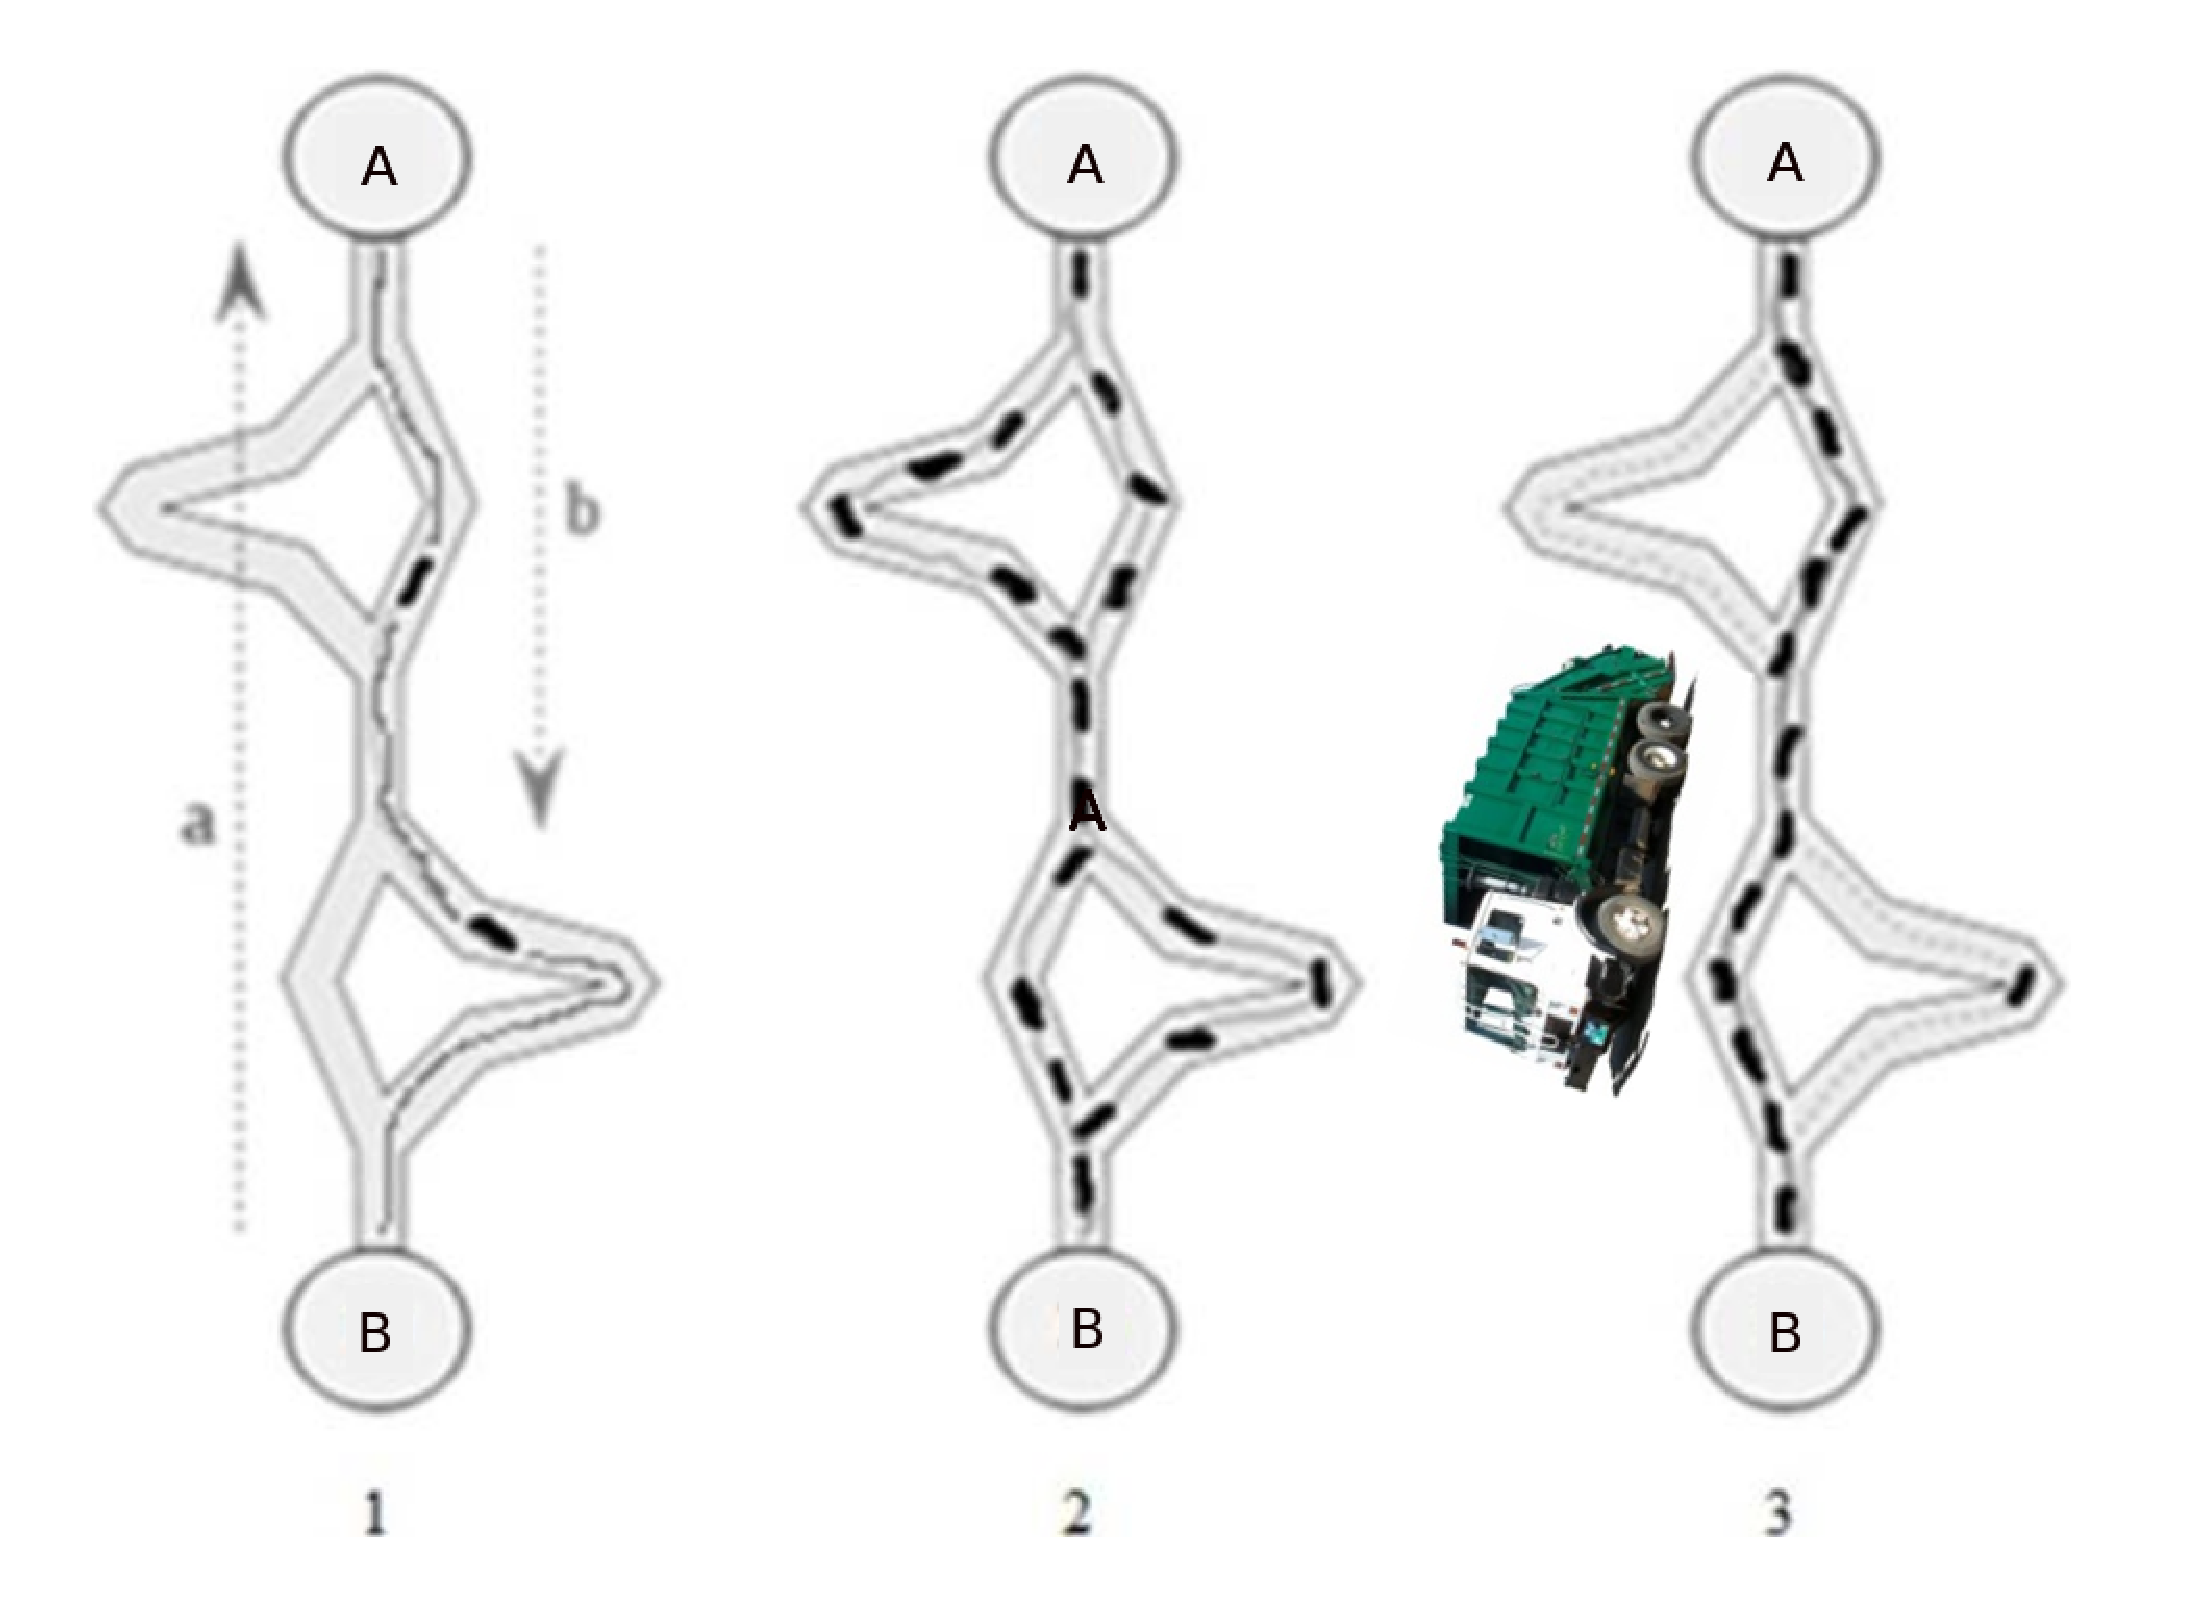
\includegraphics[%trim={3cm 4cm 3cm 3cm}, clip,
                   width=0.95\linewidth]{AntTruck}
  % figure caption is below the figure
  \caption{Three iterations of ACO}
  \label{fig:anttruck}       % Give a unique label
\end{figure}

% The PiP LevelSense™ devices include GPS location along with tilt and shock monitoring capability and temperature sensing in case of a fire. They use a battery that will last for three to five years.
% Ed Hadfield, Operations Manager at Recreational Services, the CCC contractor which manages the bins, said "The cool thing about this is that it's allowing us to utilise our resources where they're needed the most”.
% Smart Cities Programme Manager Teresa McCallum says the project shows how technology can be used to solve everyday problems.
% “We are really excited about the potential of these bin sensors to clean up an issue that causes a lot of annoyance and inconvenience to the community."

% "It is another example of the way Smart Cities is working alongside local companies to foster innovation that benefits our city and can be used throughout New Zealand and beyond. Apart from being more efficient, it’s an innovative way to make our city smarter, more sustainable, and get rid of overflowing rubbish complaints for good.”


\begin{figure*}[h]
  % Use the relevant command to insert your figure file.
  % For example, with the graphicx package use
    \centering
  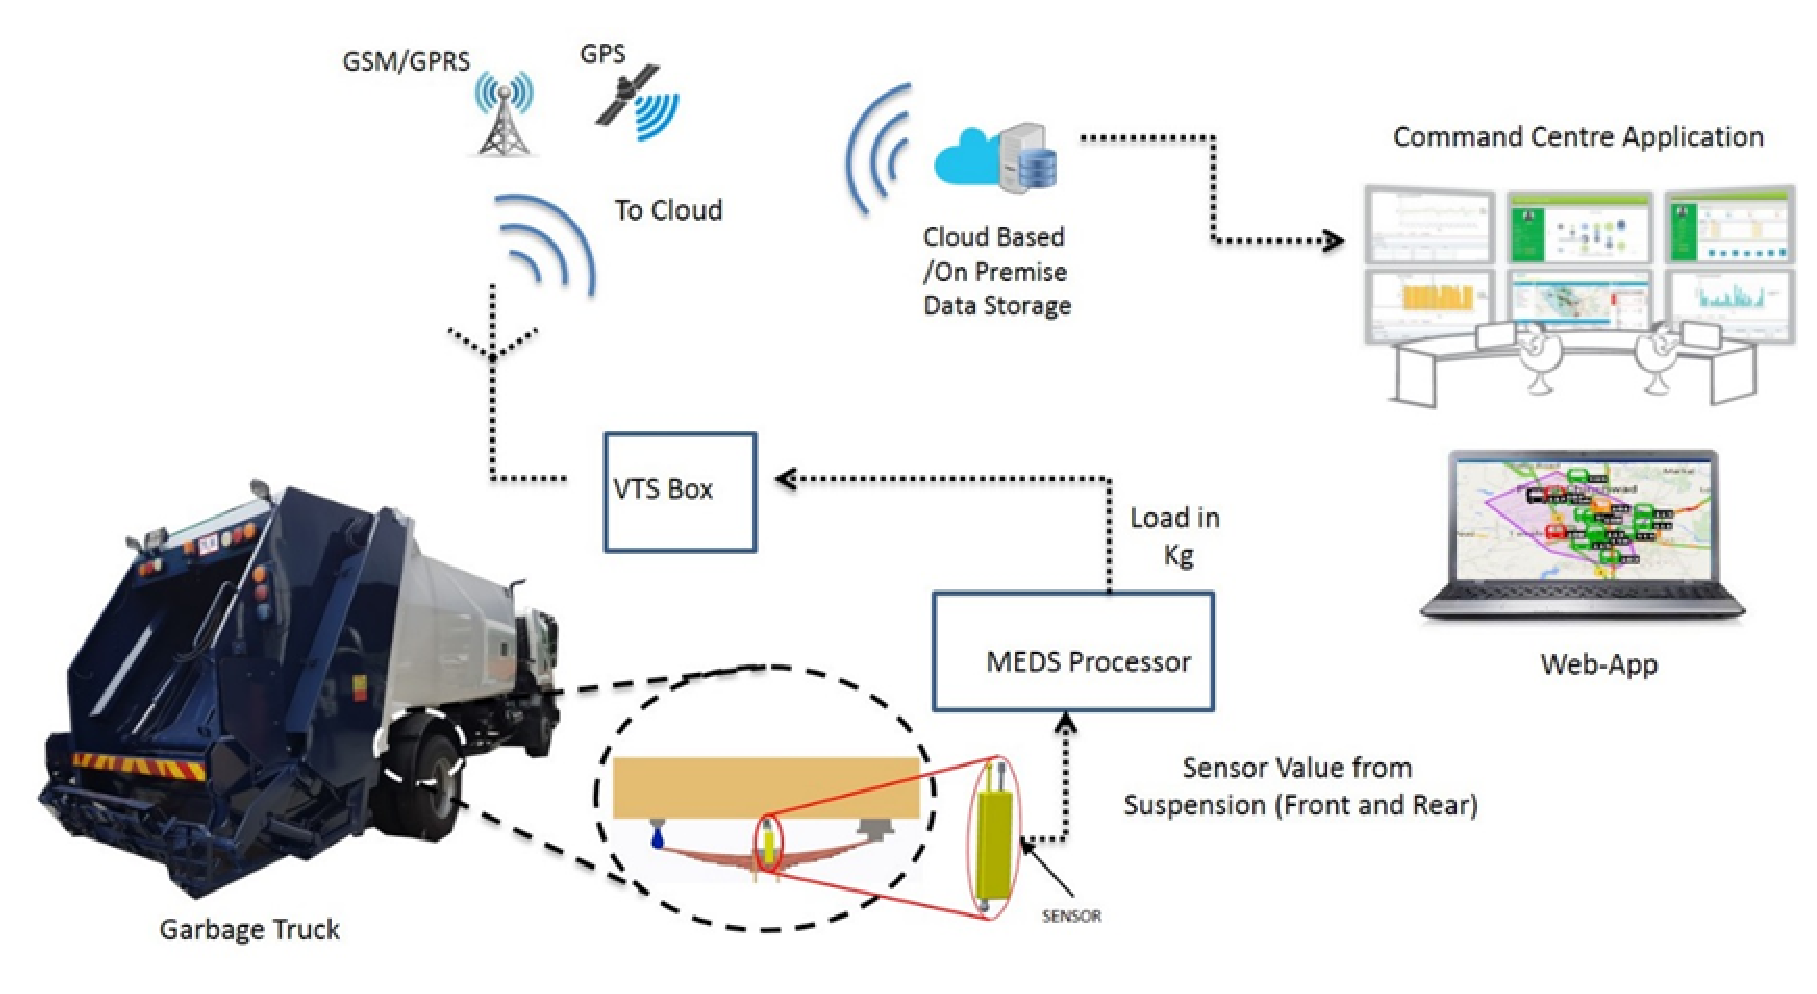
\includegraphics[%trim={3cm 4cm 3cm 3cm}, clip,
                   width=0.795\linewidth]{malaysia}
  % figure caption is below the figure
  \caption{Suspension Monitoring for Routing Malaysia's Trucks Optimally using the Greedy Approach}
  \label{fig:malaysia}       % Give a unique label
\end{figure*}

\subsubsection{Updating and Distributing Information}

For finding the optimal route connecting the full (or almost full) containers, Christchurch
pioneered in the use of ACO (Actually, the Christchurch implementation served as an 
exemplar for the Regensburg project described in section~\ref{sec:Regensburg}).
% In the traveling salesman problem, a set of cities is given and the distance between each of them is known. The goal is to find the shortest tour that allows each city to be visited once and only once. In more mathematical terms, the goal is to find a Hamiltonian tour of minimal length on a fully connected graph. In ant colony optimization, the problem is attacked by simulating a number of artificial ants moving on a graph that encodes the problem itself: each vertex represents a city and each edge represents a connection between two cities. A variable called pheromone is associated with each edge and can be read and modified by ants. Ant colony optimization is an iterative algorithm. At each iteration, a number of artificial ants are considered. Each of them builds a solution by walking from vertex to vertex on the graph with the constraint of not visiting any vertex that it has already visited in its walk. At each step of the solution construction, an ant selects the following vertex to be visited according to a stochastic mechanism that is biased by the pheromone: when in vertex i, the following vertex is selected stochastically among the previously unvisited ones. In particular, if j has not been previously visited, it can be selected with a probability that is proportional to the pheromone associated with edge (i, j). At the end of an iteration, on the basis of the quality of the solutions constructed by the ants, the pheromone values are modified in order to bias ants in future iterations to construct solutions similar to the best ones previously constructed.
% Each ant builds a solution by using

In Christchurch, the original algorithm was tuned to run on embedded devices using two types of locally accessible information: 
\begin{enumerate}
\item problem-specific information, i.e., distance among containers, and 
\item information added by ants during previous iterations of the algorithm, such as pheromone values.
\end{enumerate} 
While building a solution, each simulated ant collects information on the problem characteristics and on its own performance, and uses this information to modify the representation of the problem. The modified representation is the new environment shared by all the ants and seen locally by other ants. 
% The representation of the problem is modified in such a way that information contained in past 
% good solutions can be exploited to build new better solutions. As mentioned earlier, 
This form of indirect communication mediated by the environment is called {\it stigmergy}, and is typical of social insects~\cite{Dorigo97}).
Figure~\ref{fig:anttruck} shows how the information updates are used for
routing the garbage truck: it will take path $b$ from $A\rightarrow B$ already 
after the third iteration, since in the second iteration more simulated ants have 
returned from this path, leading to a stronger pheromone concentration than on the
longer return path $a$ from  $B\rightarrow A$.
% Suppose an ant k (in m ants) is at city i, and Nk is the set of k’s unvisited cities. Then, the ant chooses city j to visit next in a probabilistic way as follows:

% Here, η(i,j) represents the problem-specific information, and in TSP, it is the reciprocal of the distance between two cities i and j. τ(i,j) represents the information about the ant trails, i.e., the pheromone value on the route between two cities i and j. α and β are non-negative constants, and their values determine whether η (local information) or τ (global information) has more weight in the formula. τ(i,j) is updated accordingly to the following rules, when one iteration is done.

% Here, Tk represents the set of all routes from the start city to the goal city, and Lkrepresents the collective distance from the start city to the goal city. In ant-colony algorithms, the pheromone value added to a specific route is determined by the reciprocal of the total distance and the pheromone also disappears over time, where ρ represents the evaporation rate, such that newly added pheromone has more influence than old pheromone additions. Thus, after many of iterations, one can expect to obtain an approximately optimal route selection.
% As demonstrated here, ACO algorithms have been applied to dynamic versions of the TSP, where either the distance between some pairs of cities changes, or cities are dynamically added or removed from the set of cities to be visited. Additionally, an ACO algorithm has also been applied to dynamic vehicle routing problems, showing good behaviour on randomly generated problem instances and on real-world instances as well (Dorigo and Gambardella, 1997). This makes it the perfect algorithm for our dynamic waste collection vehicle routing scenario.
The waste collection problem in Christchurch poses a dynamic instance of the TSP, where cities are represented by containers and containers which are (almost) empty are not collected. Containers which are full or almost full appear in the route dashboard and 
will be collected, once a vehicle is near it.
% ACO has shown good performance on randomly generated problem instances and on real-world instances as well. This makes it the perfect algorithm for Christchurch's 
% dynamic vehicle routing scenario.

\section{The Greedy Approach to the Travelling Salesman Problem}
\label{sec:kpit}

Regensburg's project partner {\tt kpit.com} has been working on the use of TSP solvers
for vehicle routing problems in two former projects: One was focused on collecting 
waste and another one was focused on scheduling busses.

Both projects started from a brute-force method, i.\,e., a computer program that
compares all possible routes. This method was improved using a greedy approach.
Similarly to ACO, the main idea in the greedy algorithm is {\it local} optimization,
i.\,e., the algorithm picks what seems to be the best thing to do at a particular time, instead of considering the global situation. In comparison with ACO,
the greedy algorithm finds approximate solutions using a more coarsely granular
procedure leading to an increase of inaccuracy but also to an increase in performance
in many cases. 
In terms of swarm intelligence, the greedy approach is closer to the {\it Monarch
Butterfly Optimization} (MBO) than to ACO~\cite{chen17} (although our implementation
has no perturbation step). 
The greedy algorithm can be sketched as follows


\begin{enumerate}
\item Calculate transport times and distances between all stops, e.g. pickup and destination locations, as well as vehicle start locations.
\item Based on the information collected in step 1, generate routes and assign vehicles. The primary  constraint is that the total travel time for the first person to board the vehicle should not exceed 1.5 times the time taken for him to reach the destination had he chose his direct transport option.
\item 
%To go through possible options we have used simulated annealing and 
% threshold-accepting algorithms. 
For each node (stop), the eligible (satisfying time \& capacity constraints) neighbors are evaluated to form paths and the ones which meet the criteria (serve maximum demand with shortest path) are selected. The acceptance criteria considers aspects like remaining capacity, direction deviation from the destination and total travel time.
\item Since this is a greedy approach, this algorithm is susceptible to choice of first route. % and hence a customized logic is developed to 
We run it for a set of feasible origins and best possible solution (i.\,e. the one which requires the minimum number of 
resources) is chosen.
\end{enumerate}

\begin{figure*}
  % Use the relevant command to insert your figure file.
  % For example, with the graphicx package use
    \centering
  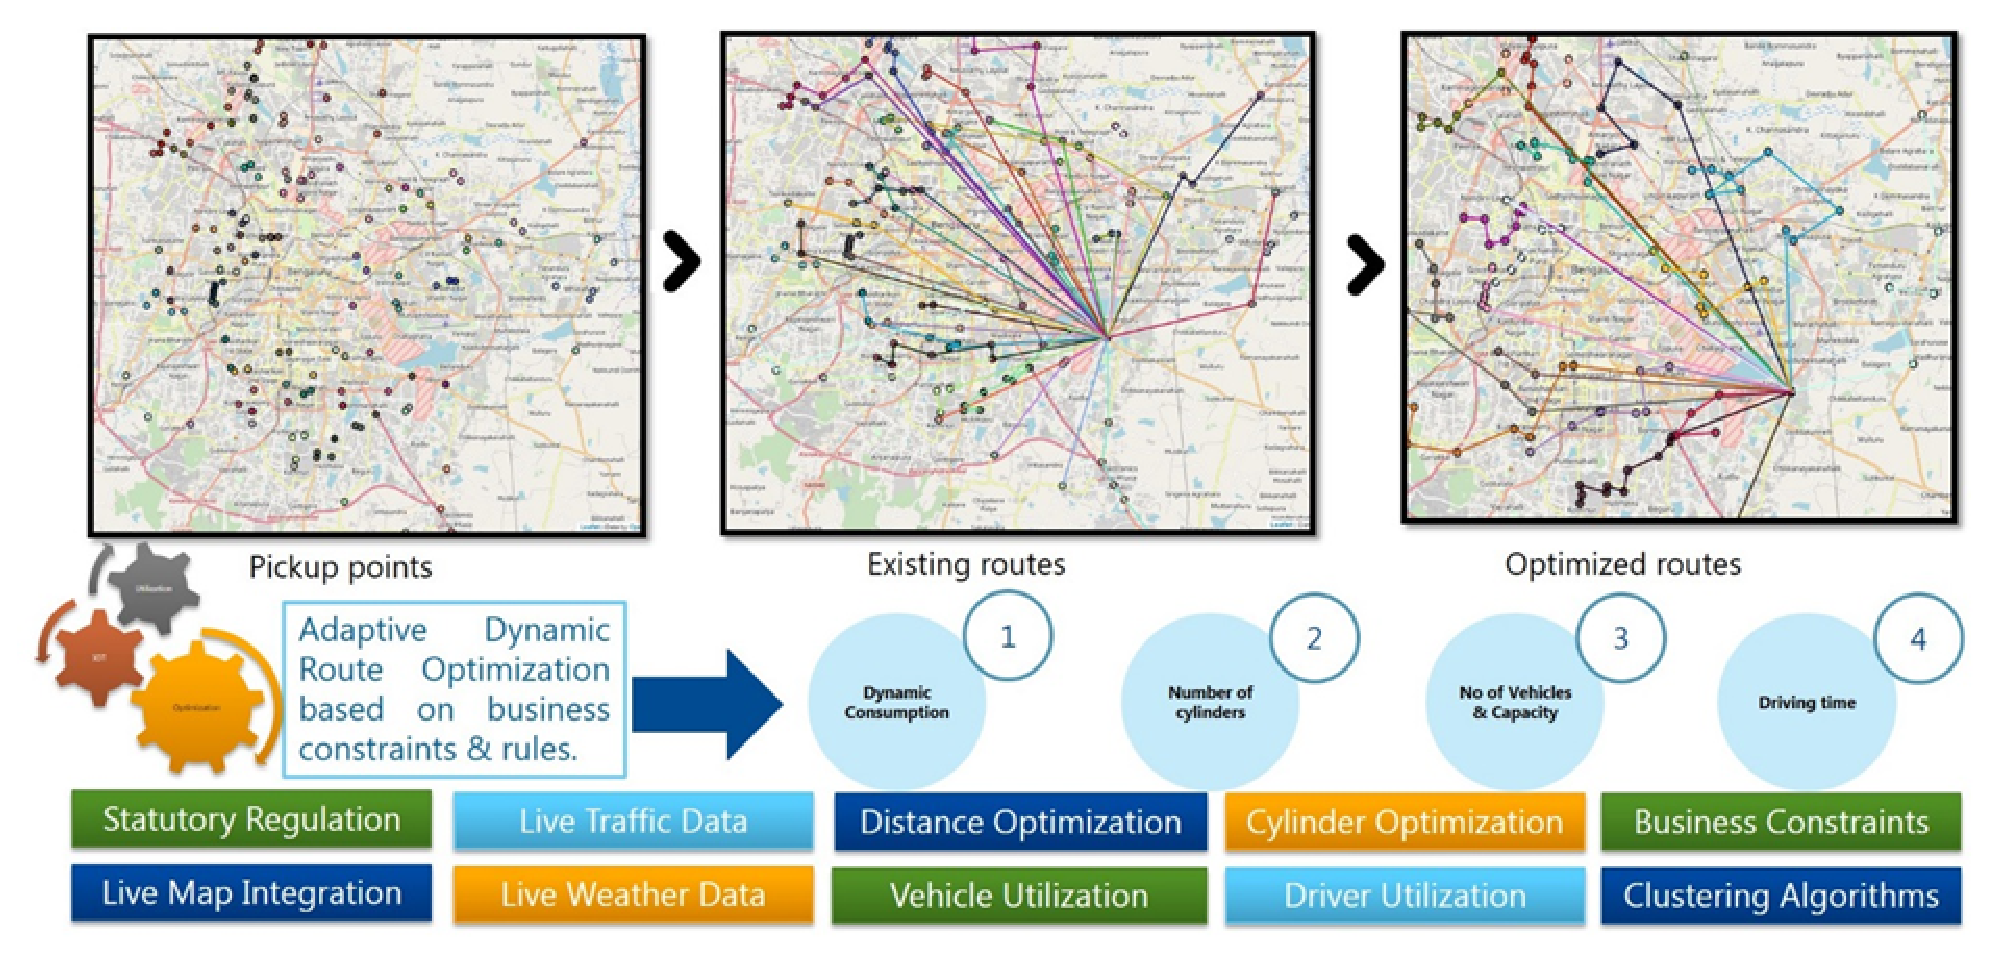
\includegraphics[%trim={3cm 4cm 3cm 3cm}, clip,
                   width=0.8795\linewidth]{employees}
  % figure caption is below the figure
  \caption{Employee collection}
  \label{fig:employees}       % Give a unique label
\end{figure*}

The first route is chosen by picking the farthest location from the office. 
We draw a circle with the office as the center and the farthest location as radius,
thus, capturing all the stops.

The above description is about routing busses collecting employees. 
However, it can be fine tuned for routing waste collection vehicles as well.
Interestingly, {\tt kpit.com} implemented this use case in Malaysia without
container sensors. Instead of monitoring the containers, the collection
vehicle load was monitored, allowing for a predictive estimation of the
container fill grades.


\subsection{Application 1: The Malaysia Garbage Initiative}
\label{sec:Malaysia}

Like New Zealand, Malaysia is another trend-setter concerning smart city activities and their garbage collection initiative is unique in multiple aspects. 
Figure~\ref{fig:malaysia} shows how the components of this IoT 
infrastructure work together: the MEDS ({\it Mechanical Engineering Design Service}) 
is was developed by {\tt kpit.com}'s engineering team to connect a microcontroller 
to the VTS ({\it Vehicle Tracking System}). This microcontroller 
converts the measured deflection on the leaf suspension to payload weight and uses 
the GSM network to transmit the data back to the backend server.

\begin{figure}[h!]
  % Use the relevant command to insert your figure file.
  % For example, with the graphicx package use
    \centering
  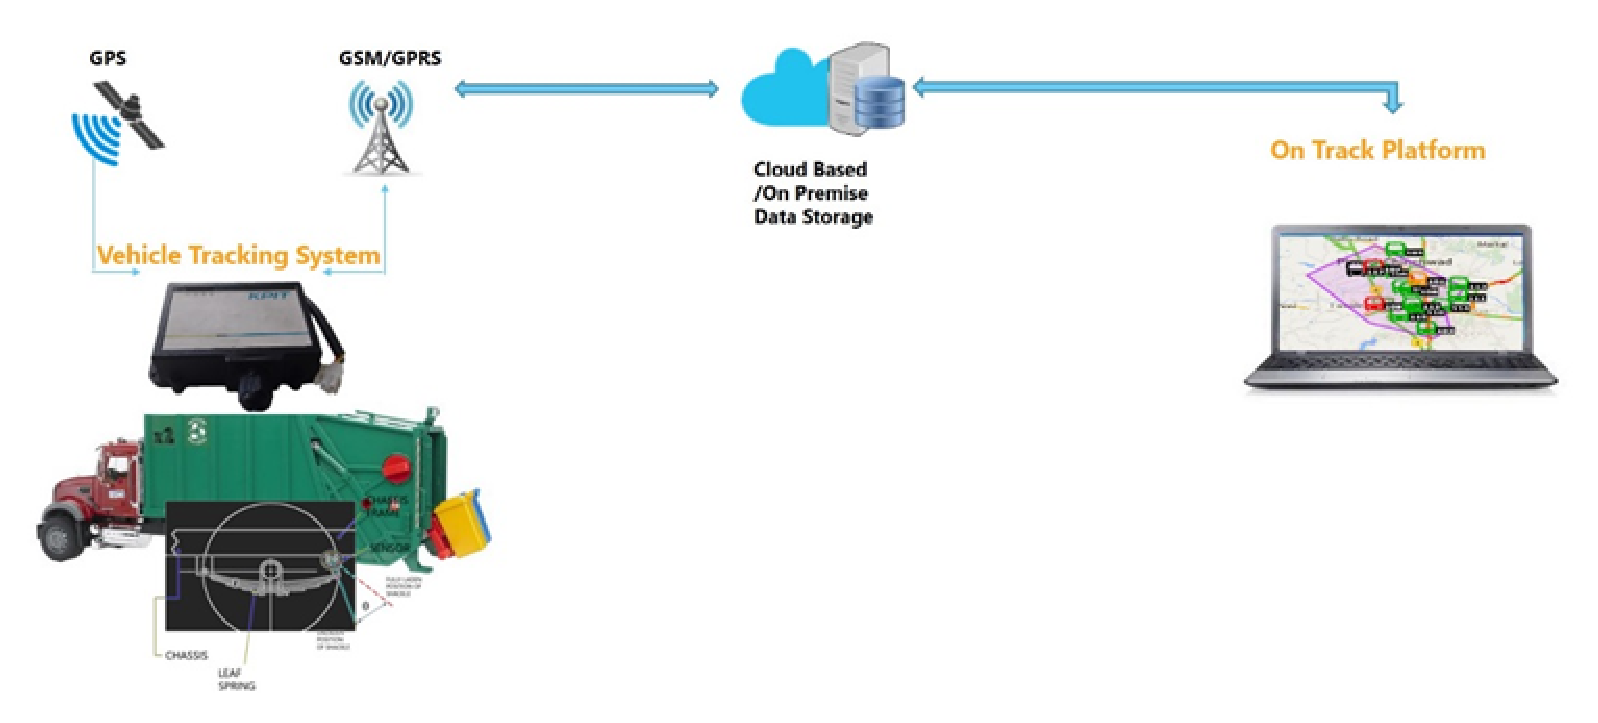
\includegraphics[%trim={3cm 4cm 3cm 3cm}, clip,
                   width=0.95\linewidth]{geofence}
  % figure caption is below the figure
  \caption{Real-time routing}
  \label{fig:geofence}       % Give a unique label
\end{figure}

The city does not only encompass the collection of garbage 
in a smart manner but it also takes into account the fleet of collection trucks and their maintenance 
to ensure availability and the necessary framework to manage the contingencies that may occur. 

For monitoring the garbage collection, Malaysia's garbage trucks are equipped with  
leaf spring sensors measuring the vehicles' suspension levels. 
The measured data and the GPS positions of the respective trucks can be visualized 
in a Web App and they are also used as input of the 
command center application for coordinating the trucks dynamically. 
The other parameters processed by this 
application comprise static information, such as the truck parking locations,
the bin locations and time estimates before a bin is full. Using these data,
the Malaysian authorities can observe the amount of the loaded garbage at each 
location, which helps them to avoid vehicle overloading and truck breakdowns.


The vehicle tracking system makes use of geo fencing to track discrepancies between the
planned and the actually driven routes (see figure~\ref{fig:geofence}). 
Comprehensive reports of every vehicle's trip history, map views and the cargo 
weight details are available in the Web App at the click of a button.


\subsection{Application 2: Optimized Bus Routing for Collecting Employees in Bangalore}
\label{sec:Bangalore}

The costs of transporting employees is a concern for many companies. Especially in India, 
where the number of employees is high in many companies these costs are huge: 
employee transport costs are the third highest cost after employee salaries and rentals.
Therefore, minimizing these costs is of vital importance.

The {\tt kpit.com} initiative was undertaken to find minimal routes and also minimize the
number of vehicles required to transport employees located at various location in the 
metro city of Bangalore. The practical implementation (sketched in 
Figure~\ref{fig:employees}) makes use of the greedy approach with the follwing setup:

\subsubsection*{Input}

\begin{itemize}
\item The demand at every stop (employees can order a bus using a smart phone App)
\item The stop locations and their positions
\item The available fleet and their corresponding capacities
\end{itemize}

\subsubsection*{Constraints}

\begin{itemize}
\item The total demand may not exceed the maximum capacity of the 39 vehicles ranging between 6 
and 30 passengers. There are 106 stops and 191 employees are using the bus transport.

\end{itemize}



%The solution approach is based on travelling salesman approach. 
% We have used the greedy approach to reduce computations and time to converge.

% \subsection{Algorithm Benchmarking}

% Collecting the waste of modern cities within the scheduled time interval is a challenging job and it is indeed a global issue.  Considering the universal aspect and the value it brings to the society, it is not only important but also cost efficient if best practices are shared to avoid reinventing the wheel.
% In this section we are benchmarking the three different solutions.



% The emerging trend of countries transitioning towards smart cities is ever-growing with the aim of enhancing the quality of living for citizens through smart technologies. And with an estimation that 66 percent of the world’s population will be living in cities by 2050, the importance of creating an improved system is crucial. Considering the population explosion that is foreseen in Asian countries, this is a major socio-economic driver.


\section{Conclusion and Future Perspectives}
\label{sec:concl}

In this work, we have analyzed and compared the vehicle routing procedures used in four practical 
smart city implementations. Our analysis has shown that the fundamental IoT approach, allowing
people to order on-demand (using their phone or a signal button at the bus stop), can be improved 
significantly by route optimization algorithms. The analysis of the waste collection projects has
also shown that the combination of processing fill level signals with route optimization leads
to the best collection times.

However, there is also a trade-off between finding the best schedule or route and taking into
account the specific requirements of a particular application. While ACO can lead to a shorter 
route than the greedy algorithm, applications like the employee collection must
cope with time windows~\cite{Kirci16}. a better utilization of busses is not no more 
beneficial, when it comes for the price of employees arriving late at work. A specific characteristic
of both, the Bangalore and the Malaysia use case was that arbitrary deviations from the  
collections plans cannot be tolerated. This additional constraint is always given,
when a route planning algorithm is applied to a vehicle with a limited load capacity
or operating distance~\cite{Wang17}.
This observation from project that were all (at least partially) implemented in 
practice distinguishes our work from simulation experiments that are often aimed
at improving route plans at all costs. The discussed experiences with the
discrepancies between theoretical and practical time savings can help
estimating the limitations of futuristic projects targeted at fully 
automatized public transport or waste collection.

Our next plans contain an improvement of the reliability of the employed 
forecasts by the use of more sensors and more detailed data (including e.\,g. 
loop ways and one-way streets). Especially in the narrow lanes of the 
Regensburg city center, the shortest way is not always the fastest and
the traveling times predicted by the Google Web service can be infeasible
for a garbage truck. However, the time saving which we could prove for all
projects let already rate all of them as a success.



% \section{References} 

% List and number all bibliographical references in 9-point Times, single-spaced, at the end of your paper. When referenced in the text, enclose the citation number in square brackets.
% % for example \cite{Jones2015,Smith2015} and \cite{Smith2015}. 
% Where appropriate, include the name(s) of editors of referenced books.

% if added before the last page, this command can help balancing columns
%\addtolength{\textheight}{-.2cm} 

%Bibliography 
\bibliographystyle{ieeetr}
\bibliography{sample}


\end{document}
